%!TEX root = main.tex
\chapter{绪论}

\section{高性能计算发展概述}

% 超算好,
自从计算机发明以来,计算,尤其是超级计算一直是人类认识自然、改造自然的一种强有力手段,具备强大计算能力的超级计算机能够有效地对各种自然现象与工程设计进行精确模拟,在科学研究、工程设计、产品研发等诸多领域起着不可替代的作用。

美国一直把超级计算作为一种事关国家安全和国家根本的重要研究领域予以重点发展。例如在新能源领域,美国阿贡实验室借助超级计算机在碳纳米管电极锂离子电池研究中取得突破性进展,让电池能量增加了近两倍,为新能源汽车的研发提供了重要支撑技术\cite{xiong2012self}。在航空航天领域,美国斯坦福大学的湍流研究中心开展了航空涡轮整机的大规模并行计算,建立了雷诺平均N-S方程与大涡模拟耦合求解的数值仿真平台,完成了约1.5亿个网格节点、4000个CPU的整机模拟\cite{reynolds2003aircraft}。在生物医药领域,英国科学与技术设施委员会与哈特里中心携手联合利华,利用高性能计算对家庭和个人护理产品的分子结构进行建模与模拟,使得开发时间从原来的8至12周缩短到45分钟\cite{Unilever}。此外,美国和欧洲的超级计算中心积极为基础研究和行业部门提供各种形式的计算服务。例如,美国XSEDE 项目通过XSEDE 工业挑战计划建立一个新的机制促进工业界和学术界之间的合作\cite{Unilever}。欧盟PRACE计划为欧洲公司提供了世界一流的高性能计算资源和服务\cite{PRACE},以提高企业竞争力,创新工业流程。

% 我国在超算上的努力
目前,我国在超级计算机系统研发方面处于国际前列,“天河二号”\cite{tianhe-2}、“神威·太湖之光”\cite{fu2016sunway}等超级计算机连续占领Top500榜首,尤其是落户于无锡太湖之滨的神威·太湖之光超级计算机首次将超级计算机的计算能力提高到百亿亿次量级\cite{fu2016sunway},很好地证明了我国在超级计算机系统研发方面的强大实力。与此同时,国内大中型企业越来越注重将高性能计算技术注入到创新过程中,高性能计算在多个重大行业领域的应用取得了长足进展,超级计算已经成为了推动诸多领域发展的重要动力。例如,中国石油东方地球物理公司利用高性能计算有效解决了“黑金”定位、油藏预测与管理等诸多技术难题\cite{luo2007hpc}。

随着科学问题的数据规模、模拟分辨率、精度需求越来越高,科学应用在高性能计算系统的计算、存储、通信和能耗等方面提出巨大的挑战,同时也促进了高性能计算的发展。在过去的十年里,超级计算机发展迅猛。例如目前世界最快的超级计算机神威·太湖之光共有10,649,600个计算核心,峰值浮点运算性能高达每秒12.5 亿亿次,其计算核心数量和运算性能分别是2005年世界最快的超级计算机BlueGene/L的81.25和456倍\cite{top5002015}。

超级计算机的体系结构在过去的40年里也发生了重大的演变,经历了向量机(Vector Machine,如Cray-I\cite{russell1978cray})、对称多处理机(Symmetric MultiProcessing,如IBM System/360\cite{anderson1967ibm})、大规模并行处理机(Massively Parallel Processing, 如IBM BlueGene\cite{adiga2002overview}))以及目前主流的集群(Cluster, 如“天河二号”\cite{tianhe-2})结构。

传统超级计算机通过提升CPU时钟频率和增大计算核心数量来提升整体计算能力,但这种方式面临着散热和能耗两大瓶颈。自2010年,一系列全新架构的处理器相继出现,如NVIDIA公司的通用计算的图形处理器\cite{nvidia2008programming}(GPGPU)和英特尔公司的Xeon Phi协处理器\cite{jeffers2013intel}。与传统的CPU架构不同,这些协处理器专注于数值计算并尽量减少甚至避免复杂的控制调度任务,可以在芯片上集成更多的轻量级计算单元,提供比传统CPU更高的运算性能。异构加速器逐渐成为高性能计算系统的重要组成部分。

\begin{table}[ht]
\centering
\caption{Top500榜单前十超级计算机系统概要(2017年11月)。}
\label{tb:top500}
\begin{tabular}{cccccc}
\hline
排名 & 国家 & 超级计算机     & 架构               & 核心数      & 持续性能        \\ \hline
1  & 中国 & 神威太湖之光     & 申威26010          & 10,649,600 & 93.0 PFlops \\ \hline
2  & 中国 & 天河二号        & Xeon + Xeon Phi    & 3,120,000  & 33.8 PFlops \\ \hline
3  & 瑞士 & Piz Daint      & Xeon + Tesla P100  & 361,760    & 19.6 PFlops \\ \hline
4  & 日本 & Gyoukou        & Xeon + PEZY-SC2    & 19,860,000 & 19.1 PFlops \\ \hline
5  & 美国 & Titan          & Cray + NVIDIA K20x & 560,640    & 17.6 PFlops \\ \hline
6  & 美国 & Sequoia        & Power BQC          & 1,572,864  & 17.1 PFlops \\ \hline
7  & 美国 & Trinity        & Cray + Xeon Phi    & 979,968    & 14.1 PFlops \\ \hline
8  & 美国 & Cori           & Cray + Xeon Phi    & 622,336    & 14.0 PFlops \\ \hline
9  & 日本 & Oakforest-PACS & CX1640 + Xeon Phi  & 556,104    & 13.5 PFlops \\ \hline
10 & 日本 & K Computer     & Fujitsu SPARC64     & 705,024    & 10.5 PFlops \\ \hline
\hline
\end{tabular}
\end{table}

近年来越来越多的超级计算平台采用异构计算架构\cite{buyya1999high},异构高性能计算平台甚至逐步取代了传统的同构超算平台。表\ref{tb:top500}展示了Top500最新(2017年11月)榜单前十的超级计算机系统,其中异构架构的超级计算机有8台,占80\%,只有美国的“Sequoia”和日本的“K Computer”超级计算机采用了同构架构。其中位列榜首的神威太湖之光超级计算机采用了我国自主研制的申威26010(SW26010)异构众核芯片,峰值性能和持续性能分别高达125 PFlops和93.0 PFlops,大幅领先其他超算;尾随其后的我国的天河二号超级计算机,它采用了Xeon + Xeon Phi异构架构,峰值性能和持续性能分别高达54.9 PFlops和33.8 PFlops。

目前高性能计算平台性能的提升一方面通过升级硬件,另一方面依赖于增加节点或加速器数量。然而,超级计算机大规模、长时间的运行给功耗提出了巨大的挑战\cite{reed2015exascale}。片上异构的处理器将任务调度单元和异构计算单元集成到同一片芯片上,有利于数据共享和降低功耗,很好地缓解了超级计算机功耗大的问题。目前TOP500榜首的“神威·太湖之光”超级计算机正是基于片上异构众核处理器\cite{fu2016sunway}——申威26010处理器(SW26010)。每个申威26010处理器具有260个核心,峰值性能为3 TFlops,与NVIDIA K80 GPU、Intel Knight Landing性能相当\cite{einkemmer2017evaluation,sodani2016knights}。“神威·太湖之光”超级计算机相对于其他超算在能耗上有很大的提升,性能功耗比为$6.05GFlops/W$,是排名第二的“天河二号”超级计算机的3.2倍。可以推测,在异构计算架构已经成为超级计算机的主流架构的同时,性能功耗比更高的片上异构众核架构也许会成为未来超级计算机发展的趋势。

另一方面,由于超算入门门槛高、应用软件开发困难、对高性能计算与应用学科交叉的要求比较高,超级计算机的应用一直处于一种“曲高和寡”的境地。而超级计算机规模在不断扩大、架构也在不断演变,这给超算的并行应用软件开发和优化带来了更严峻的挑战。近年来,不同并行开发模型相继出现,旨在降低并行软件开发和优化的难度,使超算软件能更充分发挥硬件性能。OpenMP多线程模型为用户封装了多线程调度细节,用户通过在核函数循环块前添加OpenMP指导语句对核心循环进行拆分,并调用多线程多核心并行参与计算,极大的降低了多线程编程难度。NVIDIA公司针对GPU推出通用图形处理器的编程框架CUDA\cite{cook2012cuda},使用户可以在不精通GPU硬件细节的基础上通过使用CUDA C或CUDA Fortran对GPU进行编程。NVIDIA公司为了进一步降低GPU的编程门槛,大力推广PGI编译器,用户可以使用OpenACC并行模型在核函数循环块前添加OpenACC指导语句,在不改变已有代码结构下实现GPU性能加速。与GPU相比,英特尔公司推出的众核处理器Xeon Phi的编程模型更加简单,甚至可以在少量改变或不改变CPU代码的情况下实现CPU和Xeon Phi的兼容。Xeon Phi平台在编程语言、编译器、优化工具与优化方法上都与CPU 具有很高的相似度。

不断进化的编程模型一定程度上降低了并行软件开发和优化的难度,但充分发挥高性能硬件的性能仍需要深入理解硬件结构,针对硬件架构的特性提出专门的优化方法。面对特定科学应用的大规模并行优化时,高效的性能优化方法甚至需要打破只从计算机角度进行优化的传统,而需结合科学应用算法和计算机体系结构协同优化。本文以片上异构众核架构超算——神威太湖之光为研究平台,大规模地震模拟为目标科学应用,从科学应用算法优化、异构众核体系结构优化和大规模并行优化三个层面来研究面向地震模拟应用的并行优化方法。

%例如公共集成地球系统模式(CESM)\cite{kay2015community}从1983年的大气模式开始,科学家们在前人的研究基础上不断迭代开发,30多年来在不同平台逐步累积了数百万行代码,对于移植到任意一个全新的架构都是巨大的挑战。

\section{地震模拟概述}

%地震模拟可分为天然大地震模拟和人工地震勘探模拟。天然地震是由地球板块间互相挤压碰撞而引起地表振动或破坏的自然灾害,对人们的生命财产安全造成严重的危害\cite{earthquakebaidu}。人工地震勘探模拟通过观测和分析人工地震产生的地震波在地下的传播规律,推断地下岩层的性质和形态,是地球物理勘探中最重要、解决油气勘探问题最有效的一种方法\cite{地震勘探}。地震数值模拟需要强大的算力支撑,其对高性能计算的强烈需求同时也推动着高性能计算平台的发展。

%\subsection{天然大地震模拟}

% 地震的危害
千百年来,地震一直严重威胁着人类社会的安全,它具有突发性强、破坏性高、次生灾害严重等特点。地震可以在几秒或者几十秒内造成大量的房屋倒塌和人员伤亡,其破坏性堪比一场核战争。强烈的地震通常会产生各种次生灾害,如火灾、水灾、滑坡、泥石流甚至瘟疫,这些次生灾害进一步威胁着人类社会的生命财产安全。由于突发性强、破坏力高,地震不仅对一个地区甚至一个国家的社会生活和经济活动会造成巨大的冲击,对人们的心里也造成了重大的影响。

我国位于环太平洋地震带与亚欧地震带的交汇部位,地震断裂带十分发育。中国地震局统计表明,我国陆地地震约占全球陆地地震的33\%、地震死亡人数占全球地震死亡人数的50\%以上,是一个震灾极其严重的国家\cite{地震局}。二十世纪以来,我国共发生6级以上地震近800次,涉及近30个省份,灾害面积达30多万平方千米,房屋倒塌超过700万间,死亡人数超过50万,占全国各类灾害死亡人数的54\%。其中最严重的是1976年河北省唐山市发生的7.8级大地震,直接造成了24万人死亡,16万人重伤,一座重工业城市毁于一旦,直接经济损失超过100亿元\cite{地震局}。

地震灾害对人类社会的毁灭性破坏推动着学者们孜孜不倦地研究地球内部——地震学。地震学起源于人类抵制地震的需要。公元132年,东汉著名天文学家张衡设计了地动仪,这是中国历史上最早的抗震减灾科学工作之一\citep{stein2009introduction}。如图~\ref{fig:heng-scope}所示,地动仪有八个方位,每个方位上各有龙头口含龙珠,每个龙头下方有一只蟾蜍张口等待龙珠掉落。任何一方如有地震发生,指向该方向的龙头口中的龙珠会落入蟾蜍口中,由此便可推断出发生地震的方向\cite{seismoscopewiki}。

\begin{figure}[ht]
\centering
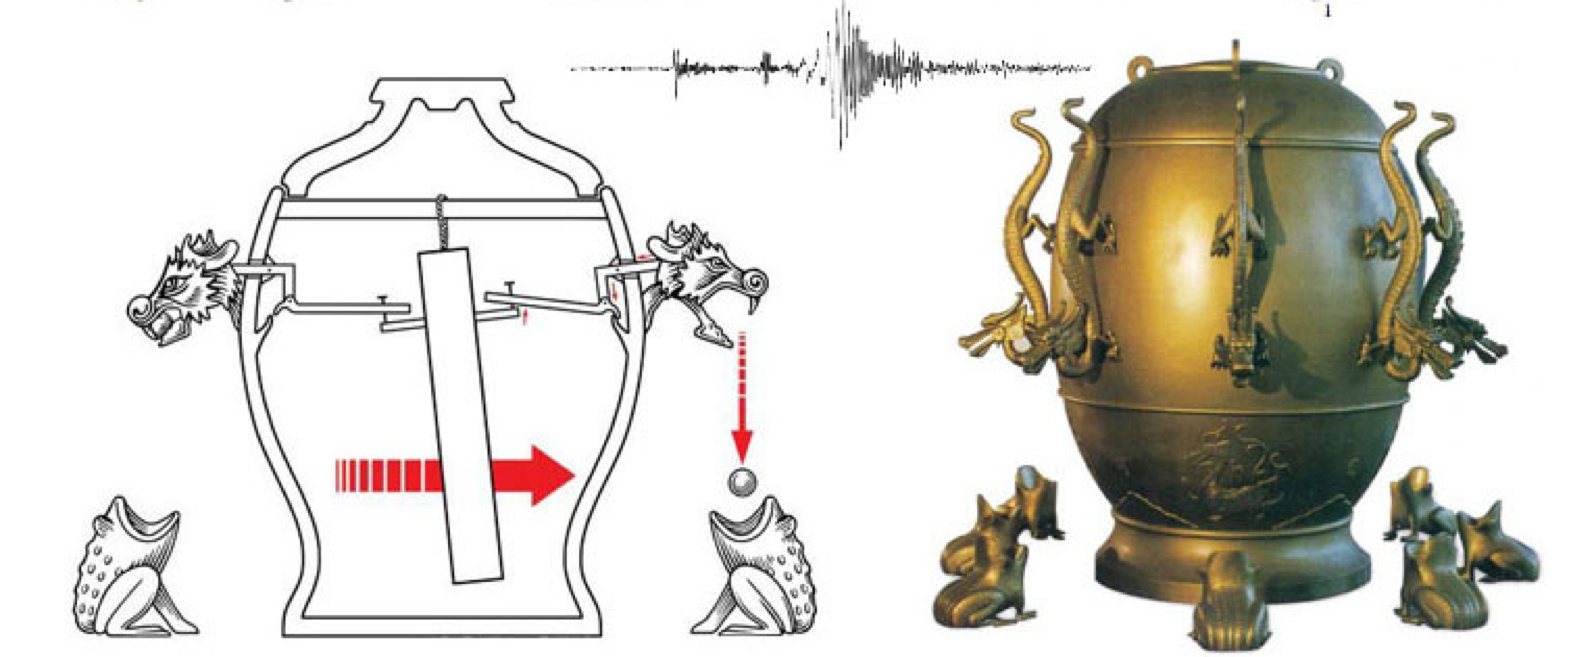
\includegraphics[width=0.7\columnwidth]{seismoscope.png}
\caption{张衡在公元132年设计的地震仪的内部结构和外观\citep{hsiao2009review}。发生地震时,指向该方向的龙头口中的龙珠会落入蟾蜍口中。}
\label{fig:heng-scope}
\end{figure}

随着20世纪科技的迅猛发展,人们发明了天然地震信号采集和测量设备,能有效地记录地震波在地球内部传播的信息。基于统计的方法逐渐成为地震风险分析和预报的主要工具。地震数值模拟工具就像一个“数字地动仪”,通过模拟地震波在地球内部的传播和地面运动,可以让科学家“模拟”甚至“预报”地震,也可以为地震相关风险提供定量评估,进一步理解地球内部结构以及地震的演变机制。此外,地震模拟工具还能够与其他科学模型(如交通、电力、水力模型)进行耦合,为地震活跃地区建立抗震救灾公用事业系统。

虽然地震数值模拟能为地震科学研究提供宝贵的“实验平台”,但它也是超级计算领域传统的“巨大挑战”。一次典型的地震模拟通常需要覆盖几百万立方米的空间范围(水平面数百公里、深度数十公里),即使计算网格空间分辨率超过100米,也会涉及数十亿到数万亿的未知数 \citep{cui2010scalable},这在过去几乎是不可解的问题。 直到最近的二三十年里,随着高性能计算的迅猛发展,基于超级计算机的地震数值模拟工具才成为了科学家研究地震的主要工具之一。

大规模地震模拟的研究工作可以追溯到1996年,Bielak等人在Cray T3D的256个处理器上使用非结构化网格进行了区域大小为$140km \times 100km \times 20km$的地震模拟\citep{bao1996earthquake},性能达到了8 Gflops。随后,日本和美国科学家相继在地球模拟器\cite{chen2006glueball}、Jaguar\cite{carrington2008high}、Cori-II\citep{breuer2017edge}和Titan\cite{cui2013physics}等超级计算机上不断研制支持范围更广、分辨率更高、模拟更精确的地震模拟工具。与此同时,随着超级计算机的规模不断扩大、架构持续更新,科学家对模拟精度、时间和空间分辨率的需求也不断提升,研制面向十亿亿次异构架构超级计算机的地震模拟工具也面临着前所未有的巨大挑战。

%\subsection{人工地震勘探}

% 意义是什么
水能覆舟亦能载舟,地震虽然给人类社会带来重大的破坏,人工的小规模地震却是开发石油天然气等化石能源的主要手段。油气资源的开采是保证国家能源供应、维持工业生产正常运行的基础,同时也是事关国民经济发展、社会稳定以及国家安全的重要因素\cite{甘霖2016面向地球科学数值模拟的可重构计算方法研究}。

在地球物理勘探中,人们通常使用地震车或空气枪制造人工地震,地震波在地下或海洋中的不同介质(如岩石、盐丘、水等)的分界处发生反射、折射(如图\ref{fig:offshoreseismicsurvey}所示\footnote{图片来源:http://oilnow.gy/exploration/ratio-announce-start-3d-seismic-work-kaieteur-block/,并进行适度修改。}),并最后被位于地表的地震数据采集阵列接收,接收到的数据被称为地震记录。通过分析人工震源函数、地震区域模型、地震记录,并采取一系列地震资料成像方法(如逆时偏移算法、全波形反演方法),人们可以反演“看到”所研究区域的地下介质分布,从而确定石油天然气等重要矿产资源的位置和产量,为后续的钻井勘探提供可行参照。

\begin{figure}[t]
  \centering
  \includegraphics[width=0.65\columnwidth]{offshoreseismicsurvey.pdf}
  \caption{地球物理勘探过程。由空气枪激发的地震波在不同介质中折射反射后到达地表接收器,并对地震资料进行处理反演地质结构,确定矿产资源的位置和产量。}
  \label{fig:offshoreseismicsurvey}
\end{figure}

石油和天然气属于不可再生资源,随着人类对于油气资源需求的不断提高,大部分简单地质下的油气资源几乎开采完毕。油气勘探的对象扩展到更加复杂的地质结构,更广阔的开采范围以及更恶劣的开采条件,石油物探技术也在不断深化和改进。自上世纪九十年代以来,石油物探的算法层面经历了Kirchhoff偏移\cite{yilmaz2001seismic}、波动方程偏移\cite{rickett2002offset},炮域波场方程偏移\cite{zhang2005theory}、逆时偏移\cite{baysal1983reverse}和全波形反演方法\cite{tarantola1984inversion};技术层面经历了从叠后到叠前,时间域到深度域,单分量到多分量,声波到弹性波,数据量和计算量都成指数增长\cite{赵改善2009高性能计算在石油物探中的应用现状与前景}。表\ref{tb:oilcomputing}预估了2003年以来石油物探地震数据处理的数据量变化以及不同偏移成像方法的计算量变化\cite{赵改善2009高性能计算在石油物探中的应用现状与前景},可以看到2015年的叠前数据量已高达180TB量级,是2005年的150倍;全波形反演算法大约需要$5\times10^{23}$次浮点运算,即便在理想情况下使用目前世界上最快的神威超算(峰值性能125PFlops)也需要一个月才能完成。未来的研究随着勘探区域和时间空间分辨率的不断提升,数据量和计算量也将进一步增长,地震资料处理对高性能计算的需求是永无止境的。

\begin{table}[ht]
\centering
\caption{地震数据处理计算量预估(浮点运算次数)}
\label{tb:oilcomputing}
\begin{tabular}{cccccc}
\hline\hline
年    份      & 2003         & 2005         & 2010         & 2015         & 未来           \\ \hline
叠前数据量       & 360GB        & 1200GB       & 30TB         & 180TB        & 700TB        \\ \hline
叠后数据量       & 12GB         & 40GB         & 600GB        & 1.8TB        & 7.2TB        \\ \hline
常规处理计算量   & $\sim1\times10^{16}$ & $\sim3\times10^{16}$ & $\sim1\times10^{18}$ & $\sim5\times10^{18}$ & $\sim2\times10^{19}$ \\ \hline
Kirchhoff偏移    & $\sim1\times10^{17}$ & $\sim3\times10^{17}$ & $\sim1\times10^{19}$ & $\sim5\times10^{19}$ & $\sim2\times10^{20}$ \\ \hline
波动方程偏移     & $\sim1\times10^{18}$ & $\sim3\times10^{18}$ & $\sim1\times10^{20}$ & $\sim5\times10^{20}$ & $\sim2\times10^{21}$ \\ \hline
炮域波动方程偏移 & $\sim1\times10^{19}$ & $\sim3\times10^{19}$ & $\sim1\times10^{21}$ & $\sim5\times10^{21}$ & $\sim2\times10^{22}$ \\ \hline
逆时偏移         & $\sim1\times10^{20}$ & $\sim3\times10^{20}$ & $\sim1\times10^{22}$ & $\sim5\times10^{22}$ & $\sim2\times10^{23}$ \\ \hline
全波形反演       & $\sim1\times10^{21}$ & $\sim3\times10^{21}$ & $\sim1\times10^{23}$ & $\sim5\times10^{23}$ & $\sim2\times10^{24}$ \\ \hline
\hline
\end{tabular}
\end{table}

\section{地震模拟在国产超算上的挑战}

地震模拟和地震资料处理对高性能计算的需求是无止境,在进一步提升地震模拟计算性能,提高模拟范围、时空分辨率、模拟精度等方面都对高性能计算提出了重大挑战。本文以目前世界上最快的神威太湖之光超级计算机为目标计算平台,总结了大规模地震模拟和地震资料处理在神威超算上开发和优化的一系列挑战。

第一个挑战是如何通过深度结合平台架构特性和目标科学应用场景,定制新的数值算法或重构算法流程以提升算法效率或模拟准确率。高性能应用优化是交叉学科研究,若不了解目标科学应用场景和具体算法流程,仅从代码的角度进行优化很容易受到原有程序算法和逻辑的制约,优化效果非常有限。若能既了解目标科学应用场景、科学原理和数值算法,又有丰富的高性能计算优化经验,便可从应用(Application)、算法(Algorithm)和体系(Architecture)三方面同时优化,拥有更大的优化空间。但这也对优化人员提出了很高的交叉学科需求。

第二个挑战是如何在申威26010异构众核处理器上将目标应用和算法的性能需求进行极致优化。更具体地说,地震模拟的核心数值算法采用的是显式有限差分方法。有限差分数值方法以计算方式规整、内存访问和节点间通信友好等优势成为了求解大规模地震波传播最常用的数值方法之一,同时该方法的性能极大的依赖于系统的内存带宽。神威太湖之光超算系统以超大的节点规模和强大的浮点运算能力著称,但其字节浮点比(float-to-byte ratio)却只有其他领先超算系统的10\%-20\%(如表\ref{tb:proc-comp}所示)。内存带宽犹如神威超算系统的一道内存墙,阻碍着地震应用性能的提升。此时需要有独特的内存相关的创新和优化才能打破神威超算的内存墙,充分发挥125 Pflops的峰值计算能力。

\begin{table}[ht]
%\footnotesize
\caption{申威26010芯片与其他多核芯片的简要对比。}
\label{tb:proc-comp}
\centering
\begin{tabular*}{0.8\columnwidth}{cccc}
\hline\hline
    芯片 & 申威26010 & Intel KNL 7250 & NVIDIA P100 \\\hline
    峰值性能 (Tflops) & 3.06 & 3 & 5.3 \\\hline
    内存技术   & DDR3 & DDR4 + MCDRAM & HBM2 \\\hline
    内存大小(GB) & 32 & 96 + 16 & 16 \\\hline
    内存带宽(GB/s)  & 136 & 102 + 460 & 732 \\\hline
\hline
\end{tabular*}
\end{table}

第三个挑战是在单节点性能优化达到极致之后,如何高效地将地震模拟从单核心和单核组扩展到神威超算上千万核心。神威超算从结构上分为节点、核组、主核和从核不同层级的处理单元,包含40,960个计算节点,每个节点内有4个核组,每个核组包含1个主核和64个从核,共10,649,600核心。如何根据不同层级处理单元的特性合理划分大规模任务,最小化不同层级处理单元间或单元内的通信、带宽和IO开销,最大化整体性能,是首要待解决问题。此外,当并行规模逐渐扩展时,应用的整体通信总量、IO总量也随之增大,通信和IO开销逐渐成为整体应用的主要瓶颈,必须针对大规模地震模拟进行特殊的通信和IO优化,才能保证地震模拟的性能高效地随着规模进行扩展。

第四个挑战是如何将上述的算法层面优化、体系结构优化和大规模并行优化技术集成到完整统一的地震模拟框架,并使用该框架或软件在神威超算上运行模拟完整真实的算例,以真实的地震模拟算例验证模拟的正确性和性能优化效果。

\section{本文工作内容与结构}

本文工作以神威太湖之光超级计算机为目标开发和优化平台,研究大规模地震模拟和地震资料处理在神威超算上的并行优化方法。根据上文提出的四大挑战,本文分别从地震正演和反演算法、申威26010处理器架构、神威超算大规模并行等角度出发提出了一系列优化方法,将地震模拟的规模、性能、分辨率和精度都推上了一个新的台阶。主要贡献包括:

\begin{itemize}
  \item 在算法层面提出了分时动态区域变分辨率正演方法和集合全波形反演方法。分时动态区域变分辨率正演方法主要利用地震波在地球内部传播时能量随着时间不断衰减的特征,使用常数衰减因子对其近似,并结合稳定性条件和频散条件,在地震波传播中不断增大时空分辨率来提升性能。该正演算法即可用于地震模拟,也可作为反演算法的基础。集合全波形反演方法以传统全波形反演方法为基础,使用集合卡尔曼滤波中的集合协方差来近似完全反演中协方差算子,并引入震源编码算法克服局部收敛、提高运算效率。集合全波形反演方法具有更大的收敛域和更低的噪音敏感度。

  \item 在体系结构层面提出了面向申威异构众核处理器的地震正演并行优化方法,分别从降低内存传输总量和提升内存传输带宽来突破申威处理器的内存墙。本文推导出最小DMA数据传输方案完成有限差分运算,并借助从核寄存器通信更新有限差分边界。在增大DMA数据传输带宽方面,本文提出了共位数组融合和数据布局转换两种方法对底层数据结构进行改动,能够显著提升DMA数据传输带宽。在内存容量达到极限的情况下,本文提出了实时压缩/解压缩方案对模拟变量进行压缩,在可接受的精度损失情况下支持更大规模的地震模拟,将应用程序的可用内存大小和带宽提升到全新的高度。

  \item 提出了面向神威超算的大规模并行优化方法。首先根据神威超算不同处理单元的特性提出了多层级并行任务划分方案,以接近线性的效率将地震模拟从单核心和单核组扩展到神威超算上千万核心。在大规模通信优化中使用额外的虚拟网格降低通信总量,并使用计算通信重叠技术隐藏通信开销。大规模并行IO优化中,本文提出了多进程串行IO方案,并使用IO分组、平衡IO和LZ4压缩提升大规模并行的IO效率。

  \item 将上述所有的优化方法整合并实现基于神威超算的地震模拟框架,并进行了非线性唐山大地震模拟和石油勘探全波形反演成像。非线性唐山大地震模拟成功地使用神威超算千万核心高效模拟了唐山大地震,该模拟的分辨率高达$8m$,性能高达$18.9PFlops$。这是世界上相同模拟区域内最大规模,最高分辨率,最精确的非线性地震模拟,并获得了2017年“戈登贝尔”奖。石油勘探集合全波形反演成像成功地反演了Marmousi模型,并与传统的全波形算法和震源编码全波形算法作比对,显示了集合全波形反演算法在性能和准确率上的优势。

\end{itemize}

后续章节主要研究内容按照以下方式进行组织:
第\ref{ch:研究现状分析}章介绍异构高性能计算和地震模拟的研究现状;
第\ref{cha:变分辨率正演与集合全波形反演方法}章提出了分时动态区域变分辨率正演方法和集合全波形反演方法在算法层面上对地震模拟进行性能优化;
第\ref{cha:面向申威异构众核处理器的并行优化方法}章提出了面向申威异构众核处理器的并行优化方法,从申威26010处理器的从核并行计算和内存带宽两方面对地震模拟进行优化;
第\ref{cha:面向神威超算系统的大规模并行优化方法}章提出了面向神威超算系统的大规模并行优化方法,根据神威超算不同处理单元的特性提出了多层级并行任务划分方案以及通信和IO优化;
第\ref{cha:地震模拟案例分析}章以算例的形式展示了基于神威超算的大规模非线性唐山大地震模拟和石油勘探全波形反演成像;
第\ref{ch:总结与展望}章是本文工作的总结与展望。



